\section{Gegen\"uberstellung der Simulations und Messergebnisse}
Ausgehend von den beschriebenen Modellierungsschritten kann nun eine sichere Evaluierung der Kurzschlussanordnungen angesetzt werden. Dabei k\"onnen die Messungen sowie das Simulationsmodell zur Kreuzvalidierung verwendet werden, sodass Mess- und Simulationsfehler weitestgehend auszuschlie\ss{}en sind. Dazu wurde das Simulationsmodell, nach den in Absatz~\ref{ch:sim} versehenen Anpassungen zun\"ach einmal zur Referenz mit den Messungen verglichen. Dazu wird zun\"achst die Testbox ohne Ringkern, jedoch mit fertigem Halterungsaufbau gegen\"ubergestellt. Abbildung~\ref{fig:boxpolycross} zeigt diese Gegen\"uberstellung.
\begin{figure}[htb]
	\centering
	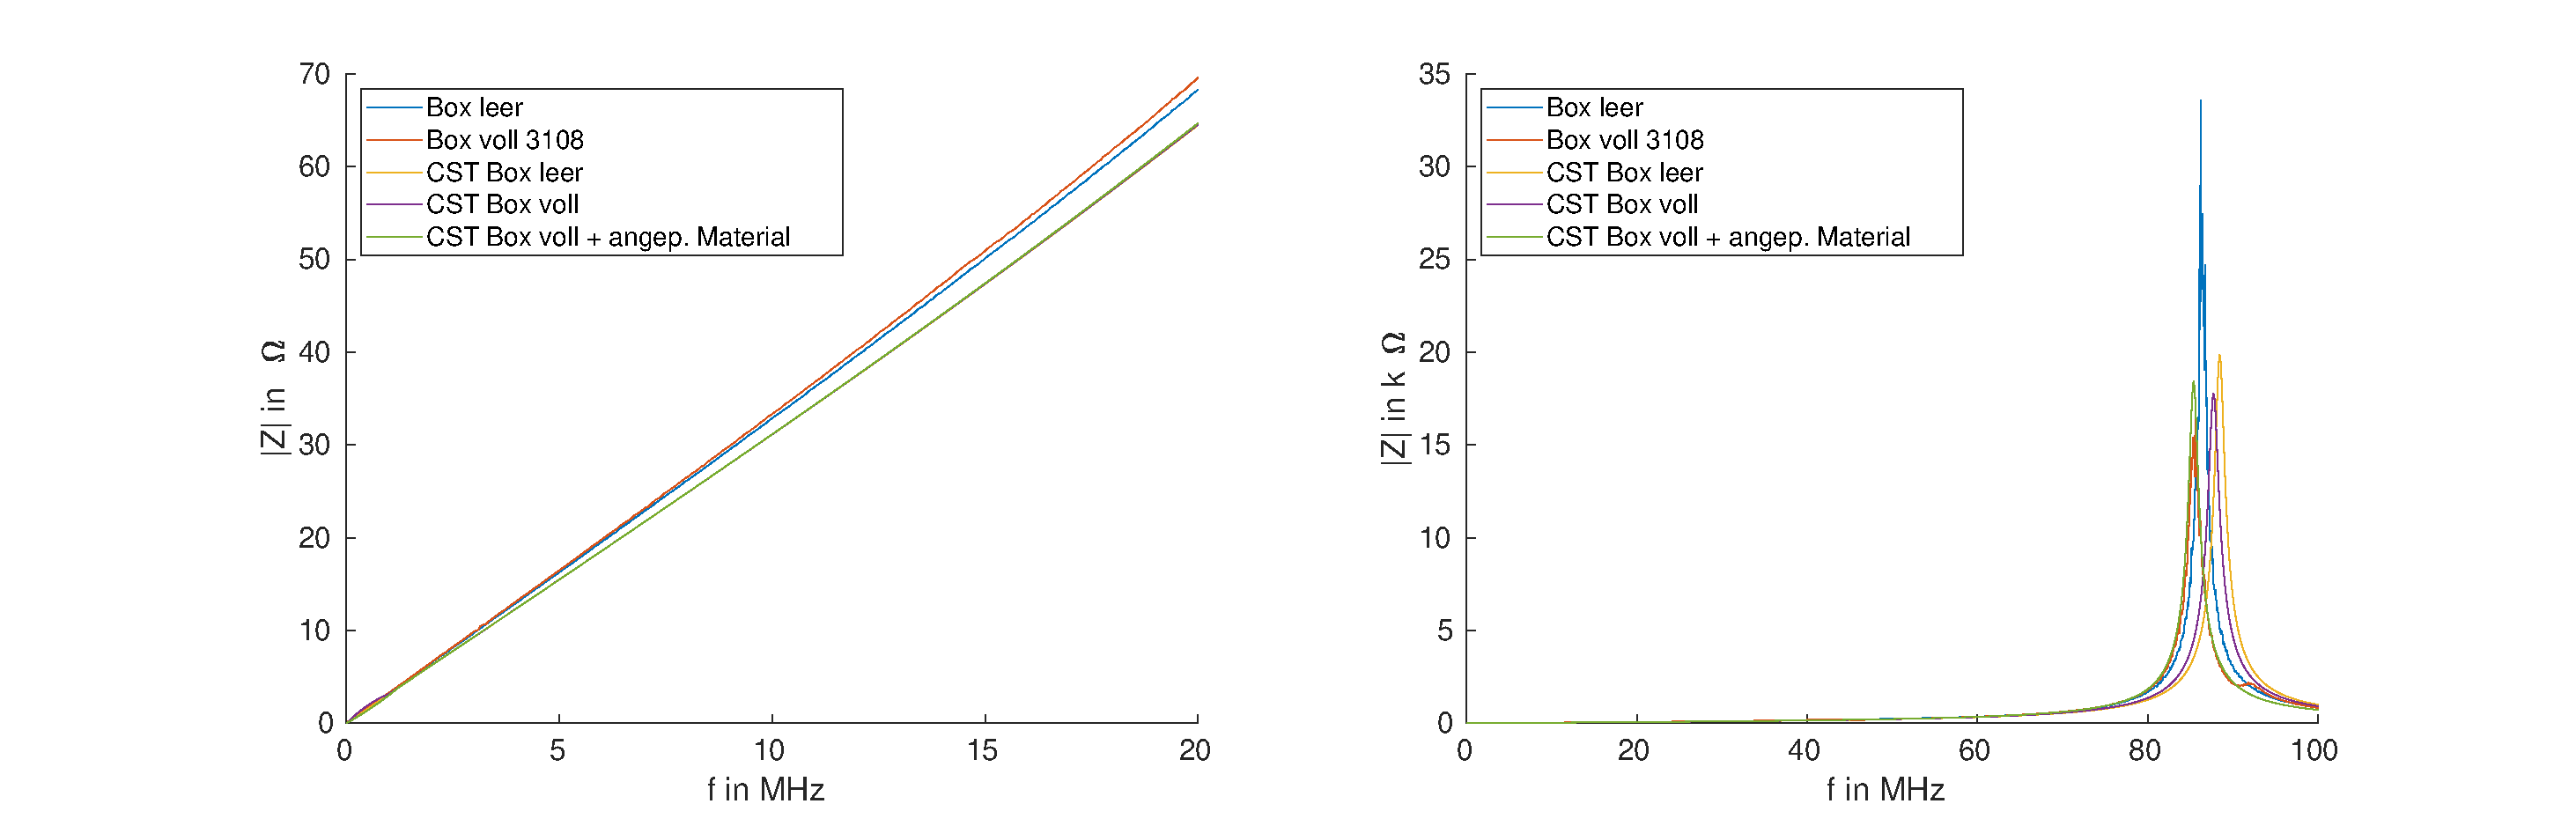
\includegraphics[width=\textwidth]{measurement_simulation_emptybox}
	\caption{Gegen\"uberstellung der Simulation der Box mit Halterung aus Kreuz und Polygon zur entsprechenden Messung.}
	\label{fig:boxpolycross}
\end{figure}
\par
Als n\"achstes in das Modell mit eingesetztem Ringkern zu evalieren. Dazu wird der Ringkern f\"ur die Simulation auf der Position um den Trovidur Ring gelegt, um die reale Box genau abzubilden. Der Aufbau ist in Abbildung~\ref{fig:RKFeRingCST} gezeigt worden. Auch hierbei wird wieder die gemessene Impedanz an der Einkopplung direkt mit der Impedanz aus der Simulation gegen\"ubergestellt. Diese Auswertung ist in Abbildung~\ref{fig:boxpolycrossrk} zu sehen.

\todo[inline,color=red!30]{Plot einf\"ugen}   

\par
Die Gegen\"uberstellung wird f\"ur alle in Abschnitt~\ref{sec:testbox} genannten Kurzschlussanordnungen in gleicher Form durchgef\"uhrt.

\par
Es zeigt sich schnell, dass insbesondere im niedrigen Frequenzbereich eine sehr geringe Abweichung zu erkennen ist. Die Mittlere Abweichung zwischen Simulation und Messung liegt unterhalb von $\SI{20}{\mega\hertz}$ bei nur \todo[inline,color=red!30]{wert und ggf Rechnung einf\"ugen}.   


\section{Auswertung der Kurzschlussanordnungen}
Nachdem die Messungen, sowie die Simulationen gegeneinander abgeglichen sind, kann die Auswertung der Kurzschlussversuche begonnen werden. Dazu wird nur die reine Ringkernimpedanz r\"uckgerechnet. Analog zum in Abschnitt~\ref{sec:ringkern} beschriebenen vorgehen, wird auch hierzu die Impedanz $Z_{rk}$ aus der gemessenen Impedanz $Z_{ges}$ nach Gleichung~\ref{eq:Zrk} herausgerechnet. Somit l\"asst sich isoliert betrachten, welcher Anteil der Ringkernimpedanz nach dem zuf\"ugen der Kurzschl\"usse noch als Rest verbleibt. Gegen\"ubergestellt werden dazu die in Unterkapitel~\ref{sec:shorts} angef\"uhrten Variationsparameter.
\par
Die maximale realtive Abweichung $a_{max}$ wird f\"ur einen Variationsparameter nach Gleichung~\ref{eq:maxdiff} berechnet.
\begin{equation}
	\frac{Z_{max} - Z_{min}}{Z_{max}} = a_{max}
	\label{eq:maxdiff}
\end{equation}
\par
Dabei entspricht $Z_{max}$ der h\"ochsten gemessenen Impedanz unter \"Anderung des Variationsparameters und $Z_{min}$ der niedrigsten. Um die relative Abweichung $a_{percent}$ in Prozent zu erhalten, wird die relative Abweichung $a_{max}E$ nach Gleichung~\ref{eq:maxdiffpercent} mit 100 multipliziert.
\begin{equation}
	\frac{Z_{max} - Z_{min}}{Z_{max}}\cdot 100 = a_{percent}
	\label{eq:maxdiffpercent}
\end{equation}


\subsection{Anzahl der Kurzschl\"usse}



\subsection{Breite der Kurzschl\"usse}
Die Breite der Kurzschl\"usse ist ein Parameter, welcher durch die Schienenartige Form der Kurzschl\"usse leicht zu variieren ist, da diese nur aus einem Blech geschnitten werden. Die Montierten Kurzschl\"usse verschiedener Breiten sind in Abbildung~\ref{fig:ringcorewidthCST} abgebildet.
\begin{figure}[htb]
	\centering
	\subfloat[$\SI{20}{\milli\meter}$]{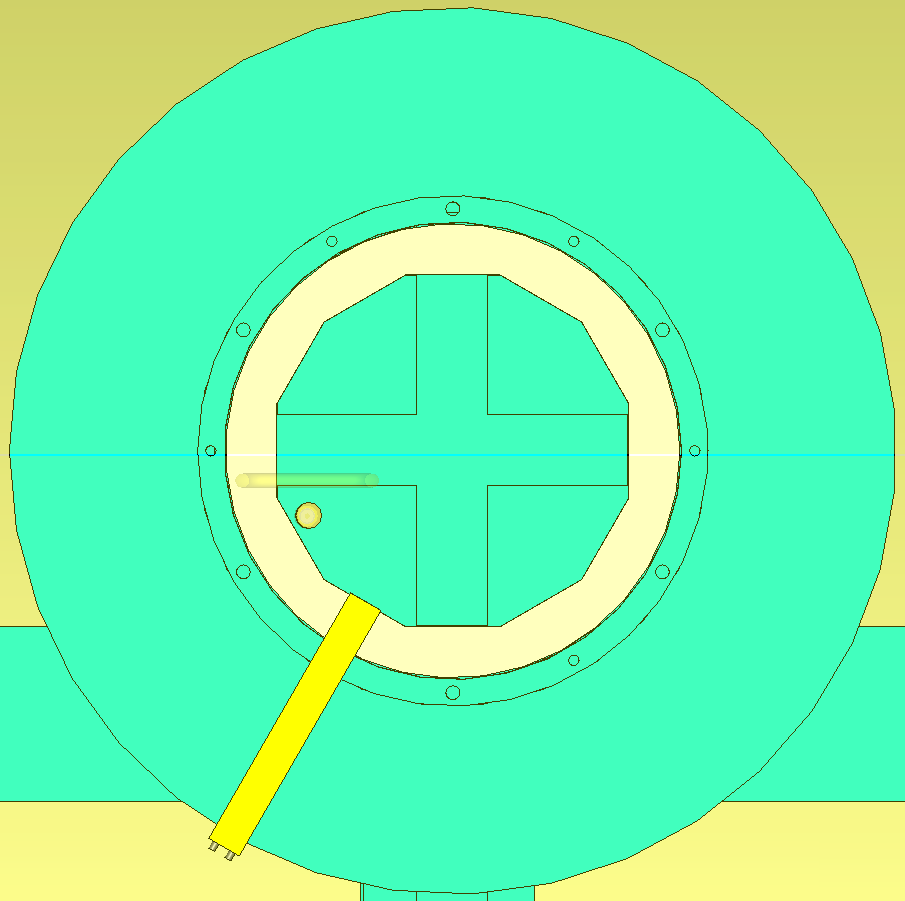
\includegraphics[height=0.3\textwidth]{1ksb20}}
	\hspace{0.02\textwidth}
	\subfloat[$\SI{30}{\milli\meter}$]{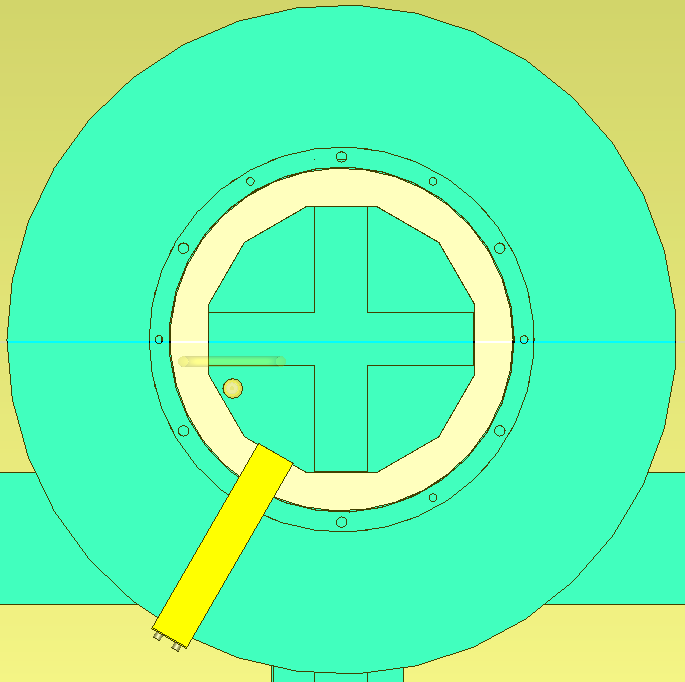
\includegraphics[height=0.3\textwidth]{1ksb30}}
	\hspace{0.02\textwidth}
	\subfloat[$\SI{50}{\milli\meter}$]{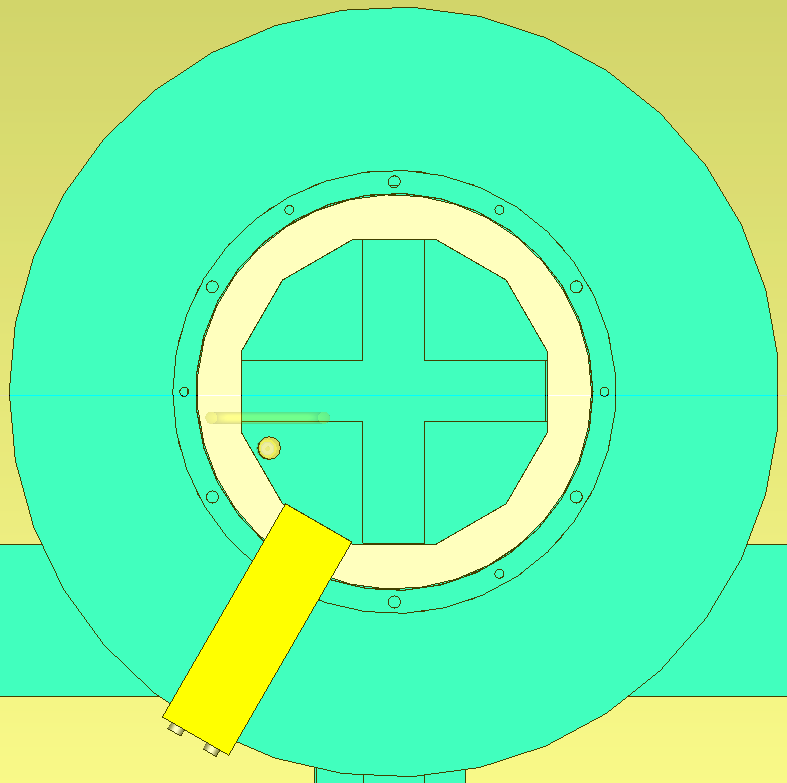
\includegraphics[height=0.3\textwidth]{1ksb50}}
	\caption{Jeweils ein montierter Kurzschluss mit verschiedenen Breiten.}
	\label{fig:ringcorewidthCST}
\end{figure}
\par
Da eine h\"ohere Anzahl an Kurzschl\"ussen eine verringerte Ringkernimpedanz als Ergebnis liefert, liegt die Vermutung nahe, dass auch breitere Kurzschl\"usse die Ringkernimpedanz weiter verringern k\"onnen. Die Gegen\"uberstellung der Ringkernimpedanz $Z_{rk}$ ist in Abbildung~\ref{fig:ringcorewidth} zu sehen.
\todo[inline,color=red!30]{Plot \"uber gesamten Frequenzbereich einf\"ugen}
\par
Auch hier wird wieder ein genaueres Augenmerk auf den relevanten Frequenzbereich unterhalb von $\SI{20}{\mega\hertz}$ gelegt. Dazu werden die Frequenzen von 5, 10 und $\SI{20}{\mega\hertz}$ geplottet und jeweils die verschiedenen Breiten gegen\"ubergestellt. Abbildung~\ref{fig:ringcorewidth20} zeigt die genannte Gegen\"uberstellung.
\begin{figure}[htb]
	\centering
	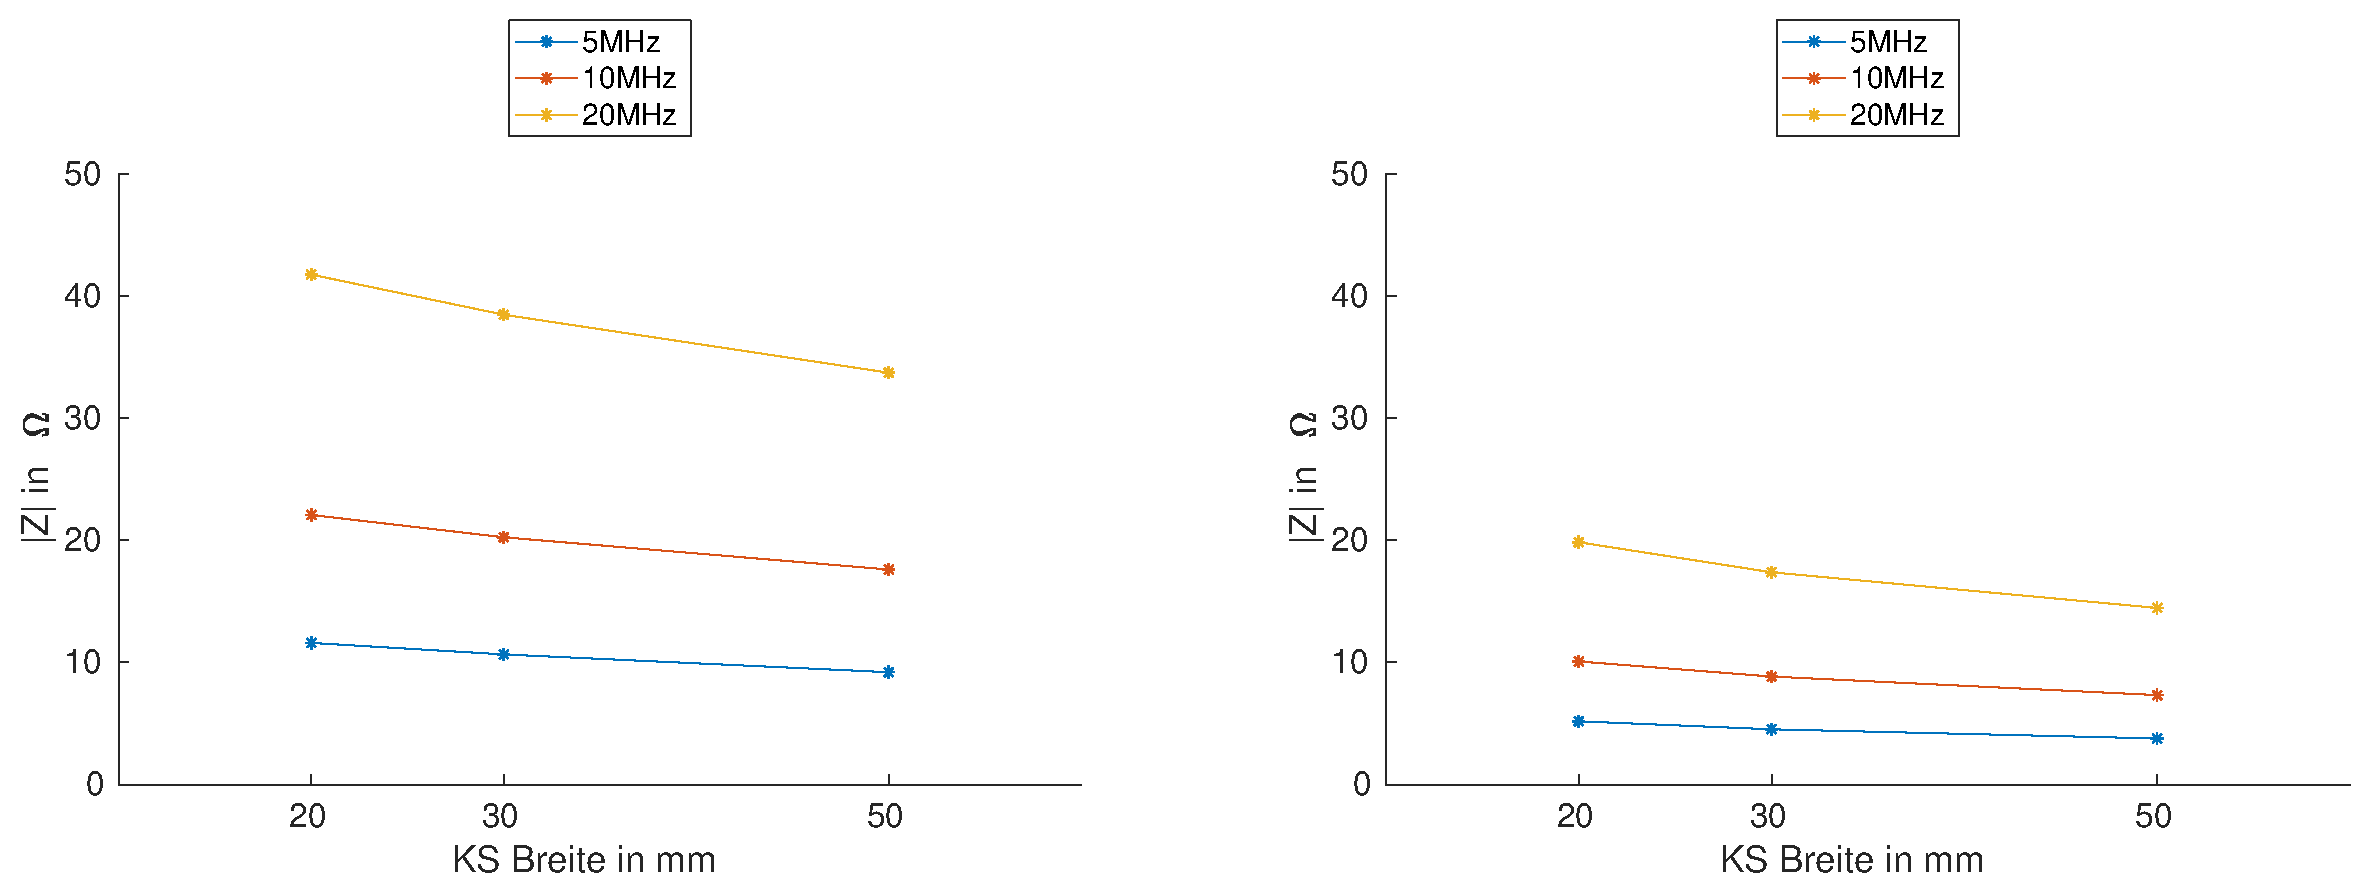
\includegraphics[width=\textwidth]{RK_Impedanz_width_frequenz}
	\caption{Gegen\"uberstellung der Ringkernimpedanz bei 5, 10 und $\SI{20}{\mega\hertz}$. Links: 1KS, rechts: 2KS.}
	\label{fig:ringcorewidth20}
\end{figure}
\par
Das Ergebnis zeigt, dass ein breiterer Kurzschluss das Ergebnis der resultierenden Ringkernimpedanz weiter verringert. Diese Variation liefert im Extremfall, also dem Unterschied von $\SI{20}{\milli\meter}$ zu $\SI{50}{\milli\meter}$ bei einer Anzahl von zwei Kurzschl\"ussen und einer Frequenz von $\SI{20}{\mega\hertz}$, eine Verringerung der Ringkernimpedanz nach Gleichung~\ref{eq:maxdiffpercent} von rund $\SI{26}{\%}$.


\subsection{L\"ange der Kurzschl\"usse}